\section{Introduction}
\subsection{Motivation}
\begin{frame}<1>[label=motivation]\frametitle{Motivation}
\begin{itemize}
	\item<1-> Neuron reconstruction
	\item<2-> Open science
	\item<3-> BigNeuron
\end{itemize}
\end{frame}

\af{2}{motivation}
\af{3}{motivation}
\begin{frame}\frametitle{BigNeuron}
	\centering
	
\includegraphics[height=0.3\textheight]{gfx/present/alleninsitute12}
\end{frame}
\begin{frame}\frametitle{BigNeuron}
	\centering
	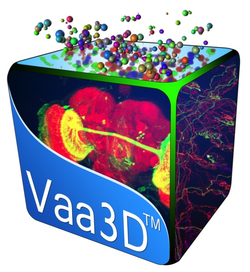
\includegraphics[height=0.5\textheight]{gfx/present/vaa3d-logo}
	\note{
		Standardising on Vaa3D image analysis tool
	}
\end{frame}
\begin{frame}\frametitle{BigNeuron}
	\centering
	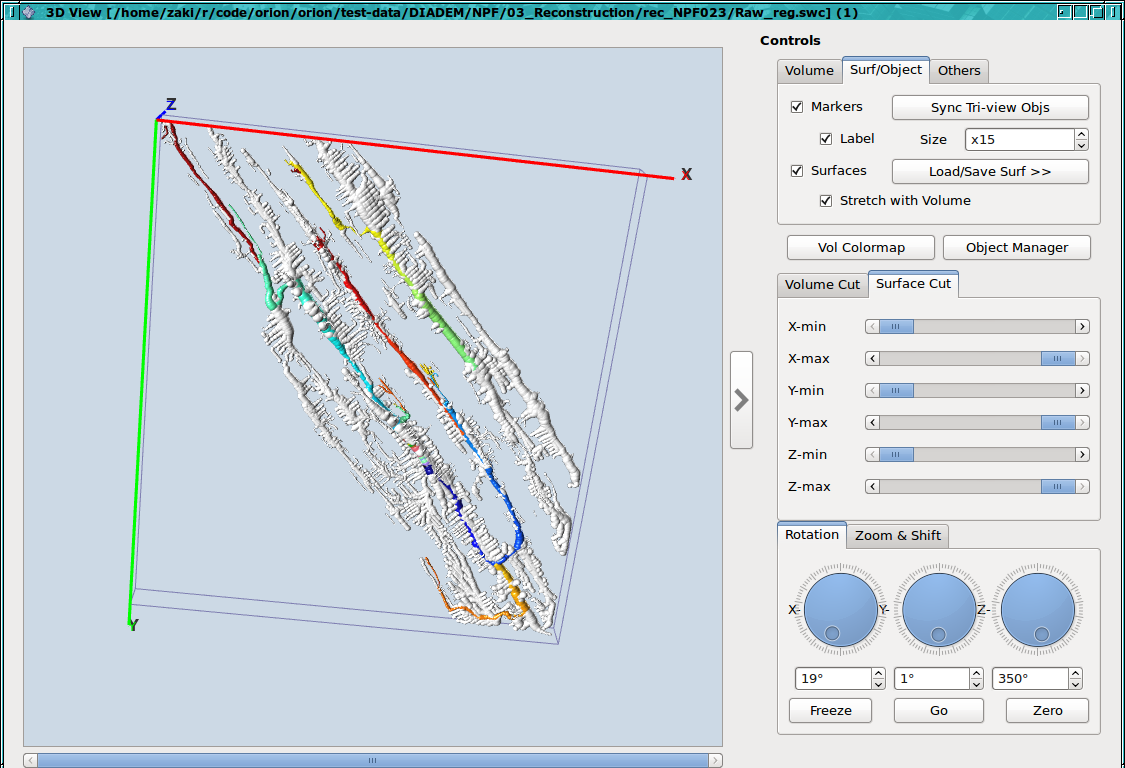
\includegraphics[height=0.5\textheight]{gfx/present/vaa3d-load-swc}
	\note{
		This is a neuron tracing loaded into Vaa3D.
	}
\end{frame}

\subsection{Objectives}
\begin{frame}<1>[label=obj]
\frametitle{Objectives}
\begin{itemize}
	\item<1> Convert the MATLAB code to C / C++
	\item<2> Integrate with Vaa3D tool for biomedical image analysis
	\item<3> Build a test suite
	\item<4> Ensure reproducibility
\end{itemize}
\end{frame}

\begin{frame}\frametitle{Conversion}
	\begin{itemize}
	\item
	  Rewrite: \textcolor{red!50}{difficult}
	\item
	  Refactor: \textcolor{green!80}{preferred}
	\item
	  Middle ground: conversion \arrowright refactor
	\end{itemize}
	\note{
		\begin{itemize}
		\item
		  Rewrites are difficult

		  \begin{itemize}
		  \item
		    They are behind time before they have been begun.
		  \item
		    You can lose some of the knowledge gained by fixing bugs.
		  \end{itemize}
		\item
		  Try to convert the code as closely as possible, then refactor into a
		  more modular architecture.
		\end{itemize}
	}
\end{frame}

\af{2}{obj}
\begin{frame}\frametitle{Vaa3D plugin}
	\centering
	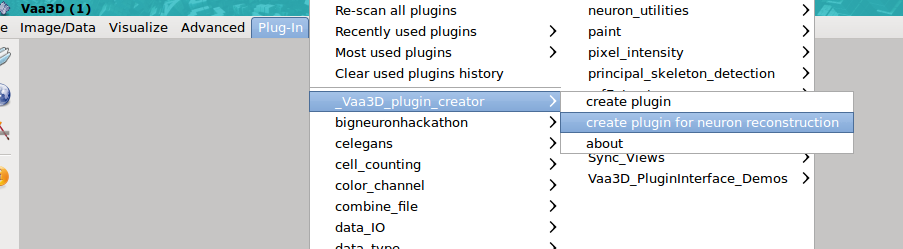
\includegraphics[height=0.3\textheight]{gfx/present/vaa3d-create-neuron-rec-plugin}
	\note{
		The idea behind contributing an algorithm to
		BigNeuron is to create a plugin that will take
		data in a standarised form and give back a
		reconstruction in a standardised form.
	}
\end{frame}

\af{3}{obj}
\begin{frame}\frametitle{Test suite}
% TODO
	\begin{itemize}
	\item
	  Encodes what the code is expected to do
	\item
	  Executable documentation
	\item
	  Helps detect regressions
	\end{itemize}
	\note{
		\begin{itemize}
			\item
				Programmers are not perfect.
			\item
				Even if we are perfect, other programmers that we interface with are
				not perfect.
			\item
				When moving to a new system, pinpoint the differences or at least get
				a starting point for debugging
			\item This leads into the reproducibility objective
		\end{itemize}
	}
\end{frame}

\af{4}{obj}
\begin{frame}\frametitle{Reproducibility for computational science}
	\begin{itemize}
	\item
	  Much of modern science is computational
	\item
	  SSI survey of researchers:

	  \begin{itemize}
	  \item
	    56\% code
	  \item
	    21\% of those: no training in software
	  \end{itemize}
	\item
	  RETRACTIONS
	\item
	  Unit tests not validation tests
	\item
	  Test many environments
	\end{itemize}
	\note{
		\begin{itemize}
		\item Note that the number is lowered since this include
			non-STEM fields. The numbers are as high as 85\% in STEM.
		\item
		  Give example of chemistry handedness mistake in protein structure
		  analysis.
		\item
		  Test step-by-step, not just look to see if the results look right
		\end{itemize}
	}
\end{frame}

\section{Analysis}

\subsection{Challenges}
\begin{frame}<1>[label=challenges]\frametitle{Challenges and risks}
\begin{itemize}
	\item<1> Reimplement MATLAB Toolbox functions
	\item<2> Memory management
	\item<3> Data layout differences of $n$-dimensional arrays
	\item<4> Data handling
\end{itemize}
	\note{
		\begin{itemize}
		\item
		  Reimplementing means having to recreate the behavior of MATLAB code
		  \emph{without} having access to the source
		\item
		  garbage collected memory vs.~manual memory management
		\end{itemize}
	}
\end{frame}

%\af{1}{challenges}
%\af{2}{challenges}
\af{3}{challenges}
\begin{frame}\frametitle{Data layout (indices)}
	\centering
	\begin{tabular}{|l|c|c|c|c|}
	\hline
	MATLAB    & \cellcolor{langM} x(1) & \cellcolor{langM} x(2) & \cellcolor{langM} x(3) & \cellcolor{langM} x(4) \\ \hline
	C         & \cellcolor{langC} x[0] & \cellcolor{langC} x[1] & \cellcolor{langC} x[2] & \cellcolor{langC} x[3] \\ \hline
	Data in x & \cellcolor{data} 4     & \cellcolor{data} 3     & \cellcolor{data} 2     & \cellcolor{data} 1     \\ \hline
	\end{tabular}
	\note{
		1-based arrays in MATLAB vs. 0-based arrays in C
	}
\end{frame}

\begin{frame}\frametitle{Data layout (row-major and column-major)}
	\centering
	\begin{tabular}{cc}
		MATLAB & C\\[1ex]
		x(r,c) & x[r][c]\\[1ex]
		\begin{tabular}{cc|c|c|c|}
		\backslashbox{r}{c}
		  & \cellcolor{langM} 1 & \cellcolor{langM} 2 & \cellcolor{langM} 3 \\
		\cellcolor{langM} 1 & \cellcolor{data} 1 & \cellcolor{data} 4 & \cellcolor{data} 7 \\\hline
		\cellcolor{langM} 2 & \cellcolor{data} 2 & \cellcolor{data} 5 & \cellcolor{data} 8 \\\hline
		\cellcolor{langM} 3 & \cellcolor{data} 3 & \cellcolor{data} 6 & \cellcolor{data} 9 \\\hline
		\end{tabular}
	&
		\begin{tabular}{cc|c|c|c|}
		\backslashbox{r}{c}
				    & \cellcolor{langC} 0 & \cellcolor{langC} 1 & \cellcolor{langC} 2 \\
		\cellcolor{langC} 0 & \cellcolor{data} 1 & \cellcolor{data} 2 & \cellcolor{data} 3 \\\hline
		\cellcolor{langC} 1 & \cellcolor{data} 4 & \cellcolor{data} 5 & \cellcolor{data} 6 \\\hline
		\cellcolor{langC} 2 & \cellcolor{data} 7 & \cellcolor{data} 8 & \cellcolor{data} 9 \\\hline
		\end{tabular}
	\end{tabular}
	\note{
		row-major (C/C++) vs. column-major (MATLAB, FORTRAN, R)
	}
\end{frame}

\af{4}{challenges}
\begin{frame}\frametitle{Data handling}
	\begin{itemize}[<+->]
		\item Caching
		\item Subvolume
	\end{itemize}
	\note{
		\begin{itemize}
		\item
		  Original code attempts to speed up subsequent runs by saving
		  intermediate results.
		\item
		  Breaks up large volumes into small volumes
		\item
		  This is fine, but every part of the codebase uses the same data by
		  reading from files.
		\end{itemize}
	}
\end{frame}

\begin{frame}\frametitle{Coupling via cross-cutting concerns}
	\begin{figure}[tbp]
	\centering
	%% Cross cutting concerns
\usetikzlibrary{arrows,calc}
\begin{tikzpicture}[node distance=1cm, >= triangle 60]

	\tikzstyle{process} = [draw,shape=rectangle,scale=0.7]
	\tikzstyle{data} = [draw,shape=circle,style=dashed,scale=0.5]
	%
	\node (data0)        at (0,0)              [data] {data file a};
	\node (data1)        [right=of data0]      [data] {data file b};
	\coordinate (Middle) at ($(data0)!0.5!(data1)$);

	\node (proc0)        [below left=of data0] [process] {Module 0};
	\node (proc1)        [below=of Middle] [process] {Module 1};
	\node (proc2)        [right=of proc1] [process] {Module 2};

	%\node (data_centreline) [right=of proc_trace] [data] {$\mathrm{Centerline}$};

	\draw [<-] (data0)   --  (proc0);
	\draw [<-] (data1)   --  (proc0);

	\draw [->] (data0)   --  (proc1);
	\draw [->] (data1)   --  (proc1);

	\draw [->] (data0)   --  (proc2);
	\draw [->] (data1)   --  (proc2);
%
\end{tikzpicture}


	\caption{\textbf{Files accessed by multiple modules}
	}\label{fig:ccc}
	\end{figure}

	\note{
		\begin{itemize}
			\item
				As soon as you make changes in one, you have to change the others.
			\item
				Imagine changing the file name
			\item
				Writes to the file-system, so it will needs file locking if run in
				parallel
		\end{itemize}
	}
\end{frame}

\begin{frame}\frametitle{Reducing coupling via indirection}
	\begin{figure}[tbp]
	\centering
	%% Cross cutting concerns solved with a DAO
\usetikzlibrary{arrows}
\begin{tikzpicture}[node distance=1cm, >= triangle 60]

	\tikzstyle{process} = [draw,shape=rectangle,scale=0.7]
	\tikzstyle{data} = [draw,shape=circle,style=dashed,scale=0.5]
	\tikzstyle{object} = [draw,shape=circle,style=solid,scale=0.5]
	%
	\node (dao)        at (0,0)      [object] {data access object};

	\node (data0)        [above left=of dao]              [data] {data file a};
	\node (data1)        [above right=of dao]      [data] {data file b};

	\node (proc0)        [below left=of dao] [process] {Module 0};
	\node (proc1)        [below=of dao] [process] {Module 1};
	\node (proc2)        [below right=of dao] [process] {Module 2};

	%\node (data_centreline) [right=of proc_trace] [data] {$\mathrm{Centerline}$};

	\draw [<->] (dao)   --  (data0);
	\draw [<->] (dao)   --  (data1);

	\draw [<-] (dao)   --  (proc0);
	\draw [<-] (dao)   --  (proc0);

	\draw [->] (dao)   --  (proc1);
	\draw [->] (dao)   --  (proc1);

	\draw [->] (dao)   --  (proc2);
	\draw [->] (dao)   --  (proc2);
%
\end{tikzpicture}


	\caption{\textbf{Using a data access object to reduce coupling}
	}\label{fig:ccc-dao}
	\end{figure}

	\note{
		\begin{itemize}
			\item Any problem in CS can be solved by adding another layer of indirection.
			\item Possible solution: Add another layer of indirection via a Data Access Object (DAO)
			\item Reduces coupling between business logic and persistence logic
			\item Persistence logic can be swapped out
		\end{itemize}
	}
\end{frame}

\subsection{Roads not taken}
\begin{frame}<1>[label=frost]\frametitle{Roads not taken}
\begin{itemize}
	\item<1> MATLAB Engine API
	\item<2> MATLAB Compiler Runtime
\note{
}
% TODO describe MATLAB Engine API and MATLAB Compiler Runtime
\end{itemize}
\end{frame}


\section{Design}

\begin{frame}<1>[label=design]\frametitle{Design}
\begin{itemize}
	\item<1> Call graph as an outline
	\item<2> Automated build system
	\item<3> Anticipating change
	\item<3> Available on GitHub for public visibility
\end{itemize}
\end{frame}

\begin{frame}\frametitle{Call graph outline}
\begin{figure}
\centering
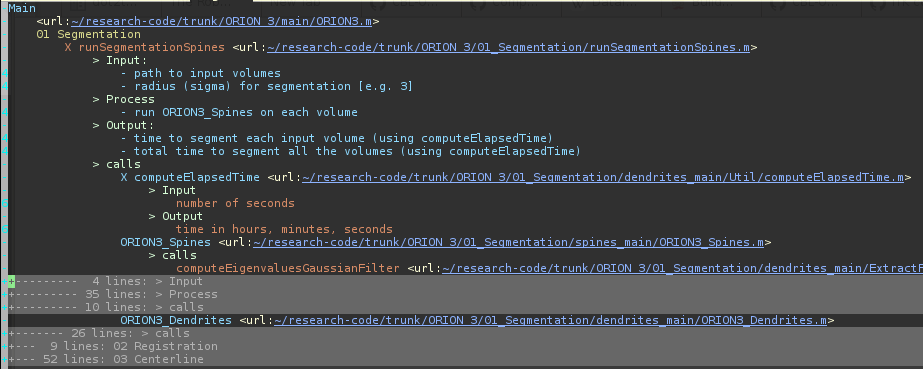
\includegraphics[width=1.0\textwidth]{gfx/call-graph-outline}
\end{figure}
\end{frame}

\begin{frame}\frametitle{Call graph visualized}
\begin{figure}
\centering
\resizebox{0.8\textwidth}{!}{\begin{tikzpicture}[node distance=0.5cm]
	\tikzstyle{step} = [draw,shape=circle,scale=0.4];
	%
	\node (step_bg_train)        at (0,0)             [draw,step] {\parbox{3cm}{\centering{}Obtain background training data}};

	\node (step_feat)        [right=of step_bg_train] [draw,step] {\parbox{2cm}{\centering{}Obtain vessellness features}};
	\node (step_discrim)     [right=of step_feat]     [draw,step] {\parbox{2cm}{\centering{}Learn discriminant function}};
	\node (step_thresh)      [below=of step_discrim]  [draw,step] {\parbox{2cm}{\centering{}Threshold}};
	\node (step_post)        [left=of step_thresh]    [draw,step] {\parbox{2cm}{\centering{}Post-processing}};

	\draw [->] (step_bg_train) -- (step_feat);
	\draw [->] (step_feat) -- (step_discrim);
	\draw [->] (step_discrim) -- (step_thresh);
	\draw [->] (step_thresh) -- (step_post);
%
\end{tikzpicture}
}
\caption[Callgraph of segmentation process in \glsentrytext{orionmat}]{
\textbf{\boldmath{} Callgraph of segmentation process in \gls{orionmat}}
}\label{fig:orionmat-segmentation}
\end{figure}
\end{frame}



\af{2}{design}
\begin{frame}\frametitle{Anticipating change}
	Directory structure
- lib
- lib/kitchen-sink
- lib/t
- src
\end{frame}

\af{3}{design}
\begin{frame}
	GNU Make-based 
	\begin{itemize}
		\item compiler extension configuration
		\item third-party library build flag configuration
		\item prerequisite scanning
	\end{itemize}
\end{frame}


\section{Implementation}

\begin{frame}
\frametitle{Implementation}
\begin{itemize}
	\item Base data structure is an n-dimensional array (row-major buffer with shape metadata)
	\item float32 for storage; float64 for calculations
	\item In-memory calculations
	\item ITK library used for implementing several filters
	\item Branch-based component development
\end{itemize}
\end{frame}

\section{Testing}

\begin{frame}
\frametitle{Testing}
\begin{itemize}
	\item Use the Test Anything Protocol (TAP) for test output
	\item Continuous integration with a pull request based workflow
	\item Automatic provisioning of build environment
	\item Tracing-based comparison to original MATLAB function
	\item Assertions for pre-/post-conditions
	\item External dependencies managed using version control
	\item Integration testing with Vaa3D plugin
\end{itemize}
\end{frame}

\section{Discussion}

\section{Conclusions}

\begin{frame}
\frametitle{Conclusions}
\begin{itemize}
	\item Software is an ever-changing system
	\item The code depends on an ecosystem
	\item Rewrites across languages are difficult
	\item Scientific software engineering is very much like traditional software engineering
	\item Open-science and reproducibility for computational methods requires software engineering skills
\end{itemize}
\end{frame}

